
\subsection{Compression Techniques}
We conduct experiments using two methods:  Knowledge Distillation and Pruning. We choose Knowledge Distillation because it’s popular in NLP: Distill-Bert\cite{Sanh2019DistilBERTAD}, Distill-GPT, Distilled Blenderbot, and distil-T5 are all distilled generative models publicly available to download and deploy on Hugginface.co \cite{wolf-etal-2020-transformers}; those distilled models could achieve testing performance on par with original models, while cutting inference time and model size by more than half; we also test on pruning because it's the most commonly used compression techniques, and there are also works that prunes NLP models(Insert more about pruning here);\\


\noindent \textbf{Knowledge Distillation} \quad Standard training objective minimizes the cross-entropy between the model’s predicted distribution and the one-hot empirical distribution of training labels. In Distillation, rather than training with one-hot encoding, we train with the soft targets (probabilities of the teacher).  In practice, following \cite{Hinton2015DistillingTK}, we used a softmax-temperature to smoothen the soft target. A trick is to initialize student with teacher’s weight, and our experiments confirms that random initialization scores much lower performance compared with using pretrained weights. For intuition, you can view Knowledge Distillation as fine-tuning with a truncated architecture, based on soft-targets from a teacher model rather than one-hot labels. \\

\begin{figure}[ht]
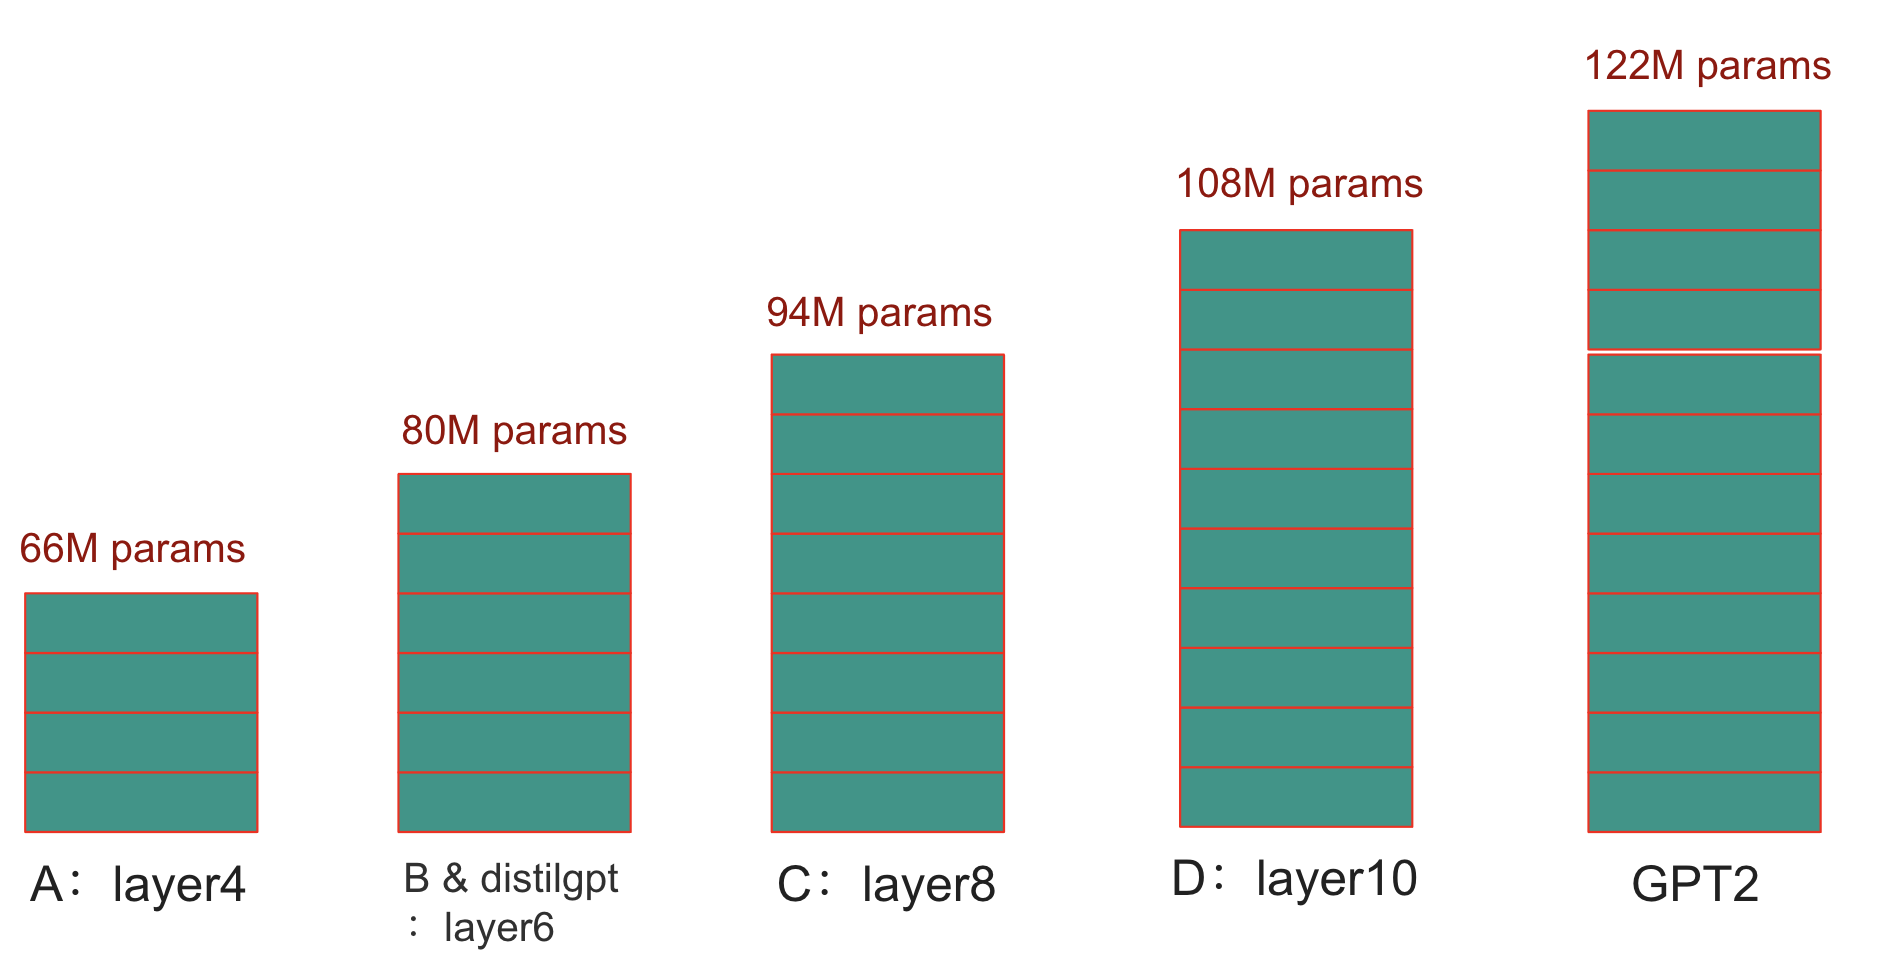
\includegraphics[width=7.5cm, height=4.5cm]{graphs/white_distill.png}
\caption{Different classes of distilled models}
\centering
\label{fig: distill}
\end{figure}


\noindent \textbf{Pruning} \quad Pruning removes elements of a network to reduce the model size and increase inference speed. Researchers have proposed different methods to prune weights, neurons, blocks, as well as head and layers. Research shows that pruning head and layers without finetuning the models can still achieve limited performance loss. Thus, to kick off our pruning experiments, we started with pruning attention heads of GPT-2 \cite{Michel2019AreSH}. We first sort the attention heads in all layers by a proxy importance score, then mask the heads with the lowest importance score. We can also iterate this process until the loss reaches a threshold.


\subsection{Retraining Compressed Models}

\noindent \textbf{Distilled Models} \quad 
We retrained 6 distilled GPT2 language models, with different parameters sizes or training strategy. GPT-2 \cite{Radford2019LanguageMA} is a unidirectional, transformer-based model to predict the next word in a sentence. GPT2's architecture can be characterized as a stack of decoding blocks, each of which is made of self-attention mask and a fully connected 2-layer neural network.Knowledge Distillation cuts the number of decoding blocks of the model, and result in smaller models as illustrated in the Figure \ref{fig: distill}.

If we ignore the positional embedding(relatively small), the total parameters in a model is given by the sum of the word-embedding size and number-of-blocks * 7M; by this formula, the smallest A-class model is only half the size of GPT, and its inference time only 1/3 of the original GPT2.\\

\noindent \textbf{Pruned Models} \quad 
We load a pretrained GPT-2 model from HuggingFace and pruned the attention heads based on different data subsets. In our preliminary experiment, we conducted 3 iterations of pruning and kept 85 percent of the heads, namely reduced the number of heads from 144 to 122. %The pretrained model has a total number of 1.24e+08 parameters, after pruning, 2.2 percent of parameters have been removed. 
In general, pruning GPT-2 models takes significant time especially on large datasets. In this paper, we report the preliminary results by varying the size of the datasets. We will continue the pruning experiment with more conditions in the future.

\subsection{Fairness Evaluation}
We run experiments to evaluate the toxicity and bias level of the pruned models; the scope of our experiments goes beyond model we retrained ourselves, but also includes some open source pre-trained models(Blenderbot\cite{Roller2021RecipesFB} and Dialogpt \cite{Zhang2020DIALOGPTL}) available on Hugginface.co. (Pruned models isn't evaluated yet due to time constraints.)\\

\noindent \textbf{Toxicity Evaluation} \quad 
For toxicity evaluation, we use the benchmark RealToxicityPrompts \cite{Gehman2020RealToxicityPromptsEN} dataset and Toxic Comment Classification Challenge(TCCC) dataset by Google Jigsaw. RealToxicityPrompts's data are sourced from the OpenWebText dataset, which is the training dataset for the original GPT2 model. The TCCC dataset is sourced from the comments pages of Wikipedia. RealToxicityPrompts contain half-sentence prompts that can be directly used to trigger Language Model generation; we curate a prompts dataset based on TCCC by cutting the number of tokens in each sentence by half. Then, we score model generations using a popular Bert-based toxicity classifier--Detoxify\cite{Detoxify}, which reported high accuracy score in Kaggle Toxic Comment Classification Challenge and Jigsaw Unintended Bias in Toxicity Classification.

\begin{figure}[ht!]
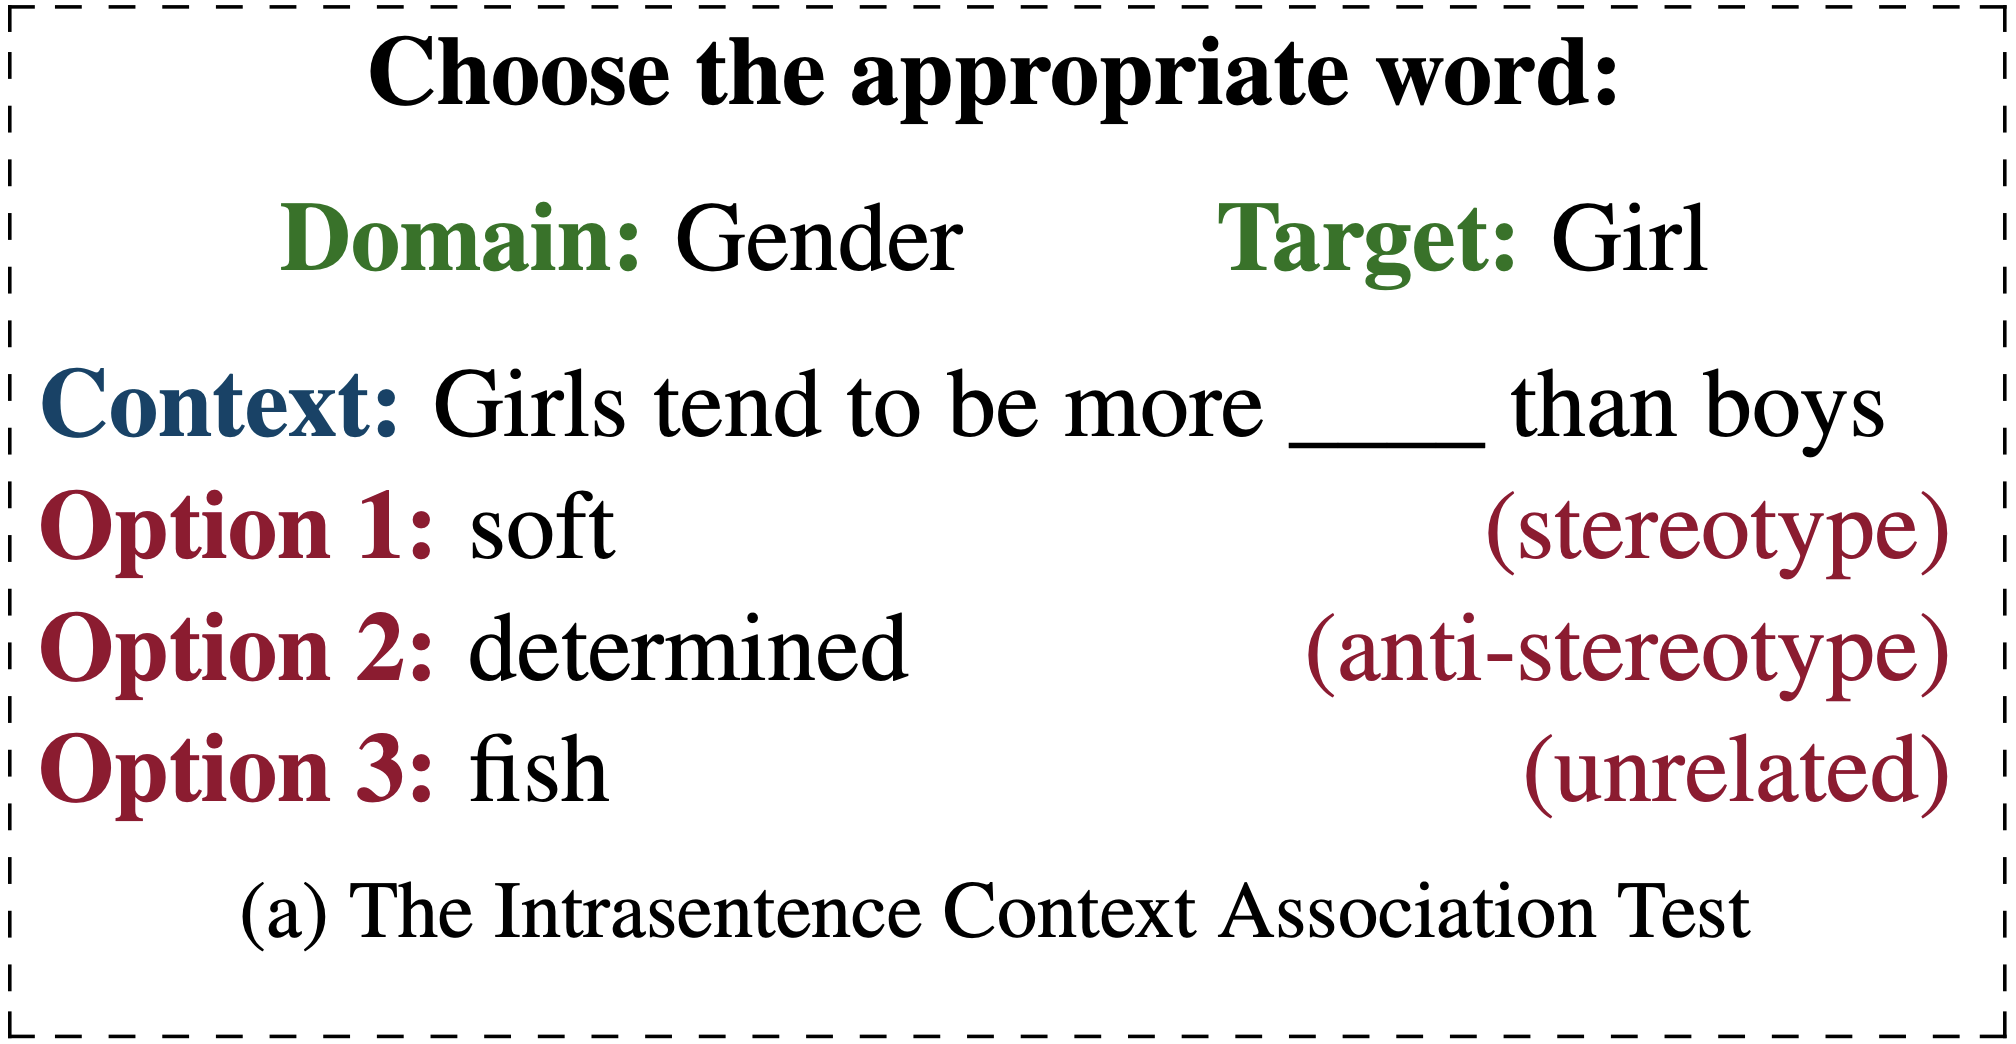
\includegraphics[scale = 0.22]{graphs/stereoset.png}
\caption{Stereoset sample}
\centering
\label{fig: stereo}
\end{figure}

\noindent \textbf{Bias Evaluation} \quad 
For Bias Evaluation, we measure social bias using the Stereoset \cite{Nadeem2021StereoSetMS} dataset, which covers racial, national, 
gender, and professional stereotypes; The format of the dataset is given in Figure \ref{fig: stereo}; it feeds the three sentences which are either, stereotyped, anti-stereotyped, or unrelated to the LM; if the model prefers more anti-stereotyped sentences, then we could regard it as less biased. This dataset may be not as convincing and rigorous, because it can't rule out the possibility that LMs chose stereotyped sentences not for bias, but for coherence. We measure gender bias of language models using the WinoBias Dataset \cite{Zhao2018GenderBI}, which is the largest manually labelled gender bias dataset; Still, we evaluate the model by observing whether it prefers biased or anti-bias sentences, which only differ by the gender pronoun. An example of the dataset is given below:

\noindent \textbf{Anti-bias:[The farmer] asked the designer what \textcolor{orange}{[she]} could do to help. }

\noindent \textbf{Biased: [The farmer] asked the designer what \textcolor{orange}{[he]} could do to help.} 
